\chapter{Results}
\label{sec:results}

\section{Baseline Results}
Baseline performance of YOLOv4 \cite{Bochkovskiy2020YOLOv4}, YOLOv8n \cite{yolov8}, and RT-DETR \cite{Zhao2023RTDETR} is measured on the three dense small-object datasets. Models are trained with the optimal hyperparameters identified during tuning. Table~\ref{tab:baseline_results} presents detection, counting, and efficiency results for later pruning comparison.

\begin{table}[t]
\centering
\caption{\textbf{Baseline detection, counting, and efficiency performance of YOLOv8n, YOLOv4, and RT-DETR across the Aedes aegypti Egg, CoNSeP, and Sorghum-Grain-Count (SGC) datasets.}}
\label{tab:baseline_results}
\resizebox{\linewidth}{!}{
  \begin{tabular}{llccccc}
\toprule
\textbf{Dataset} & \textbf{Model} & \textbf{Params (M)} & \textbf{mAP50} & \textbf{MAE} &\textbf{ Pearson's \textit{r}} & \textbf{FPS} \\
\midrule

\multirow{3}{*}{Aedes aegypti Eggs \cite{vicente2024aedesaegyptieggcounting}} 
  & YOLOv8 \cite{yolov8} & 43.63 & 0.325 & 7.10 & \textbf{0.996} & \textbf{21.38} \\
  & YOLOv4 \cite{Bochkovskiy2020YOLOv4} & 62.00 & 0.310  & 6.80  & 0.991 & 14.92 \\
  & RT-DETR \cite{Zhao2023RTDETR} & 81.00 & \textbf{0.431} & \textbf{6.20}   & 0.987 & 18.20 \\
\midrule

\multirow{3}{*}{CoNSeP \cite{Tyagi2023}} 
  & YOLOv8 \cite{yolov8} & 3.01  & \textbf{0.518} & \textbf{4.63}  & \textbf{0.925} & 32.00 \\
  & YOLOv4 \cite{Bochkovskiy2020YOLOv4} & 6.00  & 0.505 & 4.85  & 0.918 & 28.00 \\
  & RT-DETR \cite{Zhao2023RTDETR} & 31.80 & 0.495 & 5.10 & 0.912 & \textbf{38.00} \\
  \midrule

\multirow{3}{*}{SGC \cite{Bakshi2025}} 
  & YOLOv8 \cite{yolov8} & 45.00 & 0.847 & \textbf{347.2} & 0.740  & \textbf{85.00} \\
  & YOLOv4 \cite{Bochkovskiy2020YOLOv4} & 68.00 & \textbf{0.890}  & 400.0 & 0.740  & 65.00 \\
  & RT-DETR \cite{Zhao2023RTDETR} & 88.00 & 0.810 & 430.0 & \textbf{0.742} & 20.00 \\
\bottomrule
\end{tabular}

}
\end{table}

\begin{table}[p] 
\centering 
\caption{Single-Module $\Delta\text{mAP50 (\%)}$ Performance Loss Across All Models, Pruning Ratios, and Datasets.}
\scriptsize % Reduce font size
\renewcommand{\arraystretch}{0.75} % Compress vertical row spacing
\setlength{\tabcolsep}{4pt} % Compress column spacing
\label{tab:all_models_dataset_rows}
\centering
\label{tab:all_models_dataset_rows_a}
\small
\begin{tabular}{cclccc}
\toprule
& & & \multicolumn{3}{c}{\textbf{Pruned Module}} \\
\cmidrule(lr){4-6}
\textbf{Model} & \textbf{Ratio} & \textbf{Dataset} & \textbf{Backbone} & \textbf{Neck / Encoder} & \textbf{Head} \\
\midrule
\multirow{12}{*}{YOLOv8n} 
& \multirow{4}{*}{20\%} 
& Aedes a. Eggs & -0.92\% & \textbf{-2.15\%} & -1.54\% \\
& & CoNSeP        & -0.77\% & \textbf{-2.51\%} & -1.93\% \\
& & SGC           & -0.71\% & \textbf{-2.24\%} & -1.30\% \\
\cmidrule(lr){3-6}
& & \textbf{Avg. $\Delta\text{mAP50}$} & -0.80\% & \textbf{-2.30\%} & -1.59\% \\
\cmidrule(lr){2-6}
& \multirow{4}{*}{40\%} 
& Aedes a. Eggs & -4.00\% & \textbf{-6.46\%} & -5.54\% \\
& & CoNSeP        & -3.47\% & \textbf{-6.37\%} & -5.02\% \\
& & SGC           & -2.83\% & \textbf{-6.14\%} & -4.60\% \\
\cmidrule(lr){3-6}
& & \textbf{Avg. $\Delta\text{mAP50}$} & -3.43\% & \textbf{-6.32\%} & -5.05\% \\
\cmidrule(lr){2-6}
& \multirow{4}{*}{60\%} 
& Aedes a. Eggs & -9.23\% & \textbf{-15.08\%} & -12.62\% \\
& & CoNSeP        & -7.34\% & \textbf{-12.16\%} & -9.65\% \\
& & SGC           & -7.91\% & \textbf{-12.63\%} & -10.51\% \\
\cmidrule(lr){3-6}
& & \textbf{Avg. $\Delta\text{mAP50}$} & -8.16\% & \textbf{-13.29\%} & -10.93\% \\
\midrule
\multirow{12}{*}{YOLOv4} 
& \multirow{4}{*}{20\%} 
& Aedes a. Eggs & -1.29\% & \textbf{-2.58\%} & -1.94\% \\
& & CoNSeP        & -0.99\% & \textbf{-2.97\%} & -1.98\% \\
& & SGC           & -0.90\% & \textbf{-2.81\%} & -1.69\% \\
\cmidrule(lr){3-6}
& & \textbf{Avg. $\Delta\text{mAP50}$} & -1.06\% & \textbf{-2.79\%} & -1.87\% \\
\cmidrule(lr){2-6}
& \multirow{4}{*}{40\%} 
& Aedes a. Eggs & -4.52\% & \textbf{-7.42\%} & -6.45\% \\
& & CoNSeP        & -3.96\% & \textbf{-7.92\%} & -5.94\% \\
& & SGC           & -3.37\% & \textbf{-6.74\%} & -5.39\% \\
\cmidrule(lr){3-6}
& & \textbf{Avg. $\Delta\text{mAP50}$} & -3.95\% & \textbf{-7.36\%} & -5.93\% \\
\cmidrule(lr){2-6}
& \multirow{4}{*}{60\%} 
& Aedes a. Eggs & -9.03\% & \textbf{-15.48\%} & -12.90\% \\
& & CoNSeP        & -9.90\% & \textbf{-14.85\%} & -12.87\% \\
& & SGC           & -10.11\% & \textbf{-15.73\%} & -13.48\% \\
\cmidrule(lr){3-6}
& & \textbf{Avg. $\Delta\text{mAP50}$} & -9.68\% & \textbf{-15.35\%} & -13.08\% \\
\midrule
\multirow{12}{*}{RT-DETR} 
& \multirow{4}{*}{20\%} 
& Aedes a. Eggs & -1.39\% & \textbf{-3.25\%} & -1.62\% \\
& & CoNSeP        & -1.41\% & \textbf{-3.03\%} & -1.62\% \\
& & SGC           & -0.99\% & \textbf{-2.22\%} & -1.23\% \\
\cmidrule(lr){3-6}
& & \textbf{Avg. $\Delta\text{mAP50}$} & -1.26\% & \textbf{-2.83\%} & -1.49\% \\
\cmidrule(lr){2-6}
& \multirow{4}{*}{40\%} 
& Aedes a. Eggs & -4.64\% & \textbf{-8.35\%} & -5.34\% \\
& & CoNSeP        & -4.65\% & \textbf{-8.08\%} & -5.66\% \\
& & SGC           & -3.09\% & \textbf{-5.93\%} & -4.32\% \\
\cmidrule(lr){3-6}
& & \textbf{Avg. $\Delta\text{mAP50}$} & -4.13\% & \textbf{-7.45\%} & -5.11\% \\
\cmidrule(lr){2-6}
& \multirow{4}{*}{60\%} 
& Aedes a. Eggs & -10.67\% & \textbf{-19.95\%} & -13.92\% \\
& & CoNSeP        & -10.10\% & \textbf{-15.15\%} & -12.73\% \\
& & SGC           & -6.17\% & \textbf{-10.86\%} & -8.89\% \\
\cmidrule(lr){3-6}
& & \textbf{Avg. $\Delta\text{mAP50}$} & -8.98\% & \textbf{-15.32\%} & -11.85\% \\
\bottomrule
\end{tabular}
\end{table}

\subsection{Single-Module Sensitivity Analysis}

To evaluate the structural vulnerability of individual architectural components, structured channel pruning was independently applied to the Backbone, Neck (or Transformer Encoder in RT-DETR), and Detection Head across pruning ratios of 20\%, 40\%, and 60\%. The performance impact across all datasets is summarized in Table~\ref{tab:all_models_dataset_rows}. 

\subsubsection{Hierarchical Sensitivity of Architectural Modules}
Across all evaluated detection architectures (YOLOv8n, YOLOv4, and RT-DETR) and datasets, a consistent hierarchical pattern of module sensitivity emerges: 
\begin{equation}
\text{Neck / Encoder} > \text{Detection Head} > \text{Backbone}
\end{equation}

Pruning the \textbf{Neck / Encoder} yields the most severe degradation in detection accuracy ($\Delta\text{mAP50}$) across all experimental configurations. At a 20\% pruning ratio, Neck pruning causes average mAP50 drops of -2.30\%, -2.79\%, and -2.83\% for YOLOv8n, YOLOv4, and RT-DETR, respectively. As the pruning severity increases to 60\%, the performance degradation escalates sharply, resulting in average losses of -13.29\% for YOLOv8n, -15.35\% for YOLOv4, and -15.32\% for RT-DETR. The extreme sensitivity of the Neck/Encoder highlights its crucial role in feature aggregation and multi-scale feature fusion (e.g., via PANet or Transformer encoder blocks), where channel reduction severely disrupts the representation of objects at varying scales.

The \textbf{Detection Head} represents the second most sensitive component. At a 60\% pruning ratio, pruning the Head alone results in average mAP50 losses of -10.93\% (YOLOv8n), -13.08\% (YOLOv4), and -11.85\% (RT-DETR). Because the head directly maps extracted features to class predictions and bounding box regressions, aggressive channel removal here limits the capacity to output fine-grained spatial and semantic predictions.

Conversely, the \textbf{Backbone} exhibits the highest resilience to structured pruning. Even at 60\% pruning, Backbone performance losses remain significantly lower than those of the Neck or Head, averaging -8.16\% for YOLOv8n, -9.68\% for YOLOv4, and -8.98\% for RT-DETR. This indicates a high degree of channel redundancy in deep feature extraction layers, allowing pre-trained backbones to preserve critical low-level and high-level visual features even when substantial channel capacity is removed.

\subsubsection{Impact of Pruning Ratio Progression}
The transition from conservative (20\%) to aggressive (60\%) pruning ratios demonstrates a non-linear rate of performance decay:
\begin{itemize}
    \item \textbf{20\% Pruning Ratio:} All models remain highly robust, maintaining $\Delta\text{mAP50}$ losses below 3.5\% across all individual modules. For instance, YOLOv8n on the SGC dataset experiences only a minimal drop of -0.71\% for Backbone pruning and -2.24\% for Neck pruning.
    \item \textbf{40\% Pruning Ratio:} Performance loss becomes moderate but noticeable. Average Neck losses across all models range from -6.32\% to -7.45\%, marking the onset of capacity bottlenecks in multi-scale feature synthesis.
    \item \textbf{60\% Pruning Ratio:} The degradation becomes severe across all components. The peak single-module drop is observed in RT-DETR on the \textit{Aedes a. Eggs} dataset, where pruning the Transformer Encoder at 60\% leads to a sharp -19.95\% loss in mAP50.
\end{itemize}

\subsubsection{Cross-Architecture and Dataset Variability}
Comparing architectural paradigms reveals that transformer-based RT-DETR and legacy YOLOv4 suffer slightly higher peak degradation under aggressive pruning (60\% Neck pruning losses of -15.32\% and -15.35\%, respectively) compared to YOLOv8n (-13.29\%). Regarding dataset variance, tasks involving small object detection—such as \textit{Aedes a. Eggs}—exhibit higher sensitivity to Neck and Head pruning than dense cellular datasets like CoNSeP or SGC. This indicates that fine-grained spatial features required for tiny target localization are disproportionately concentrated in the multi-scale fusion layers.

\begin{figure*}[t]
\centering
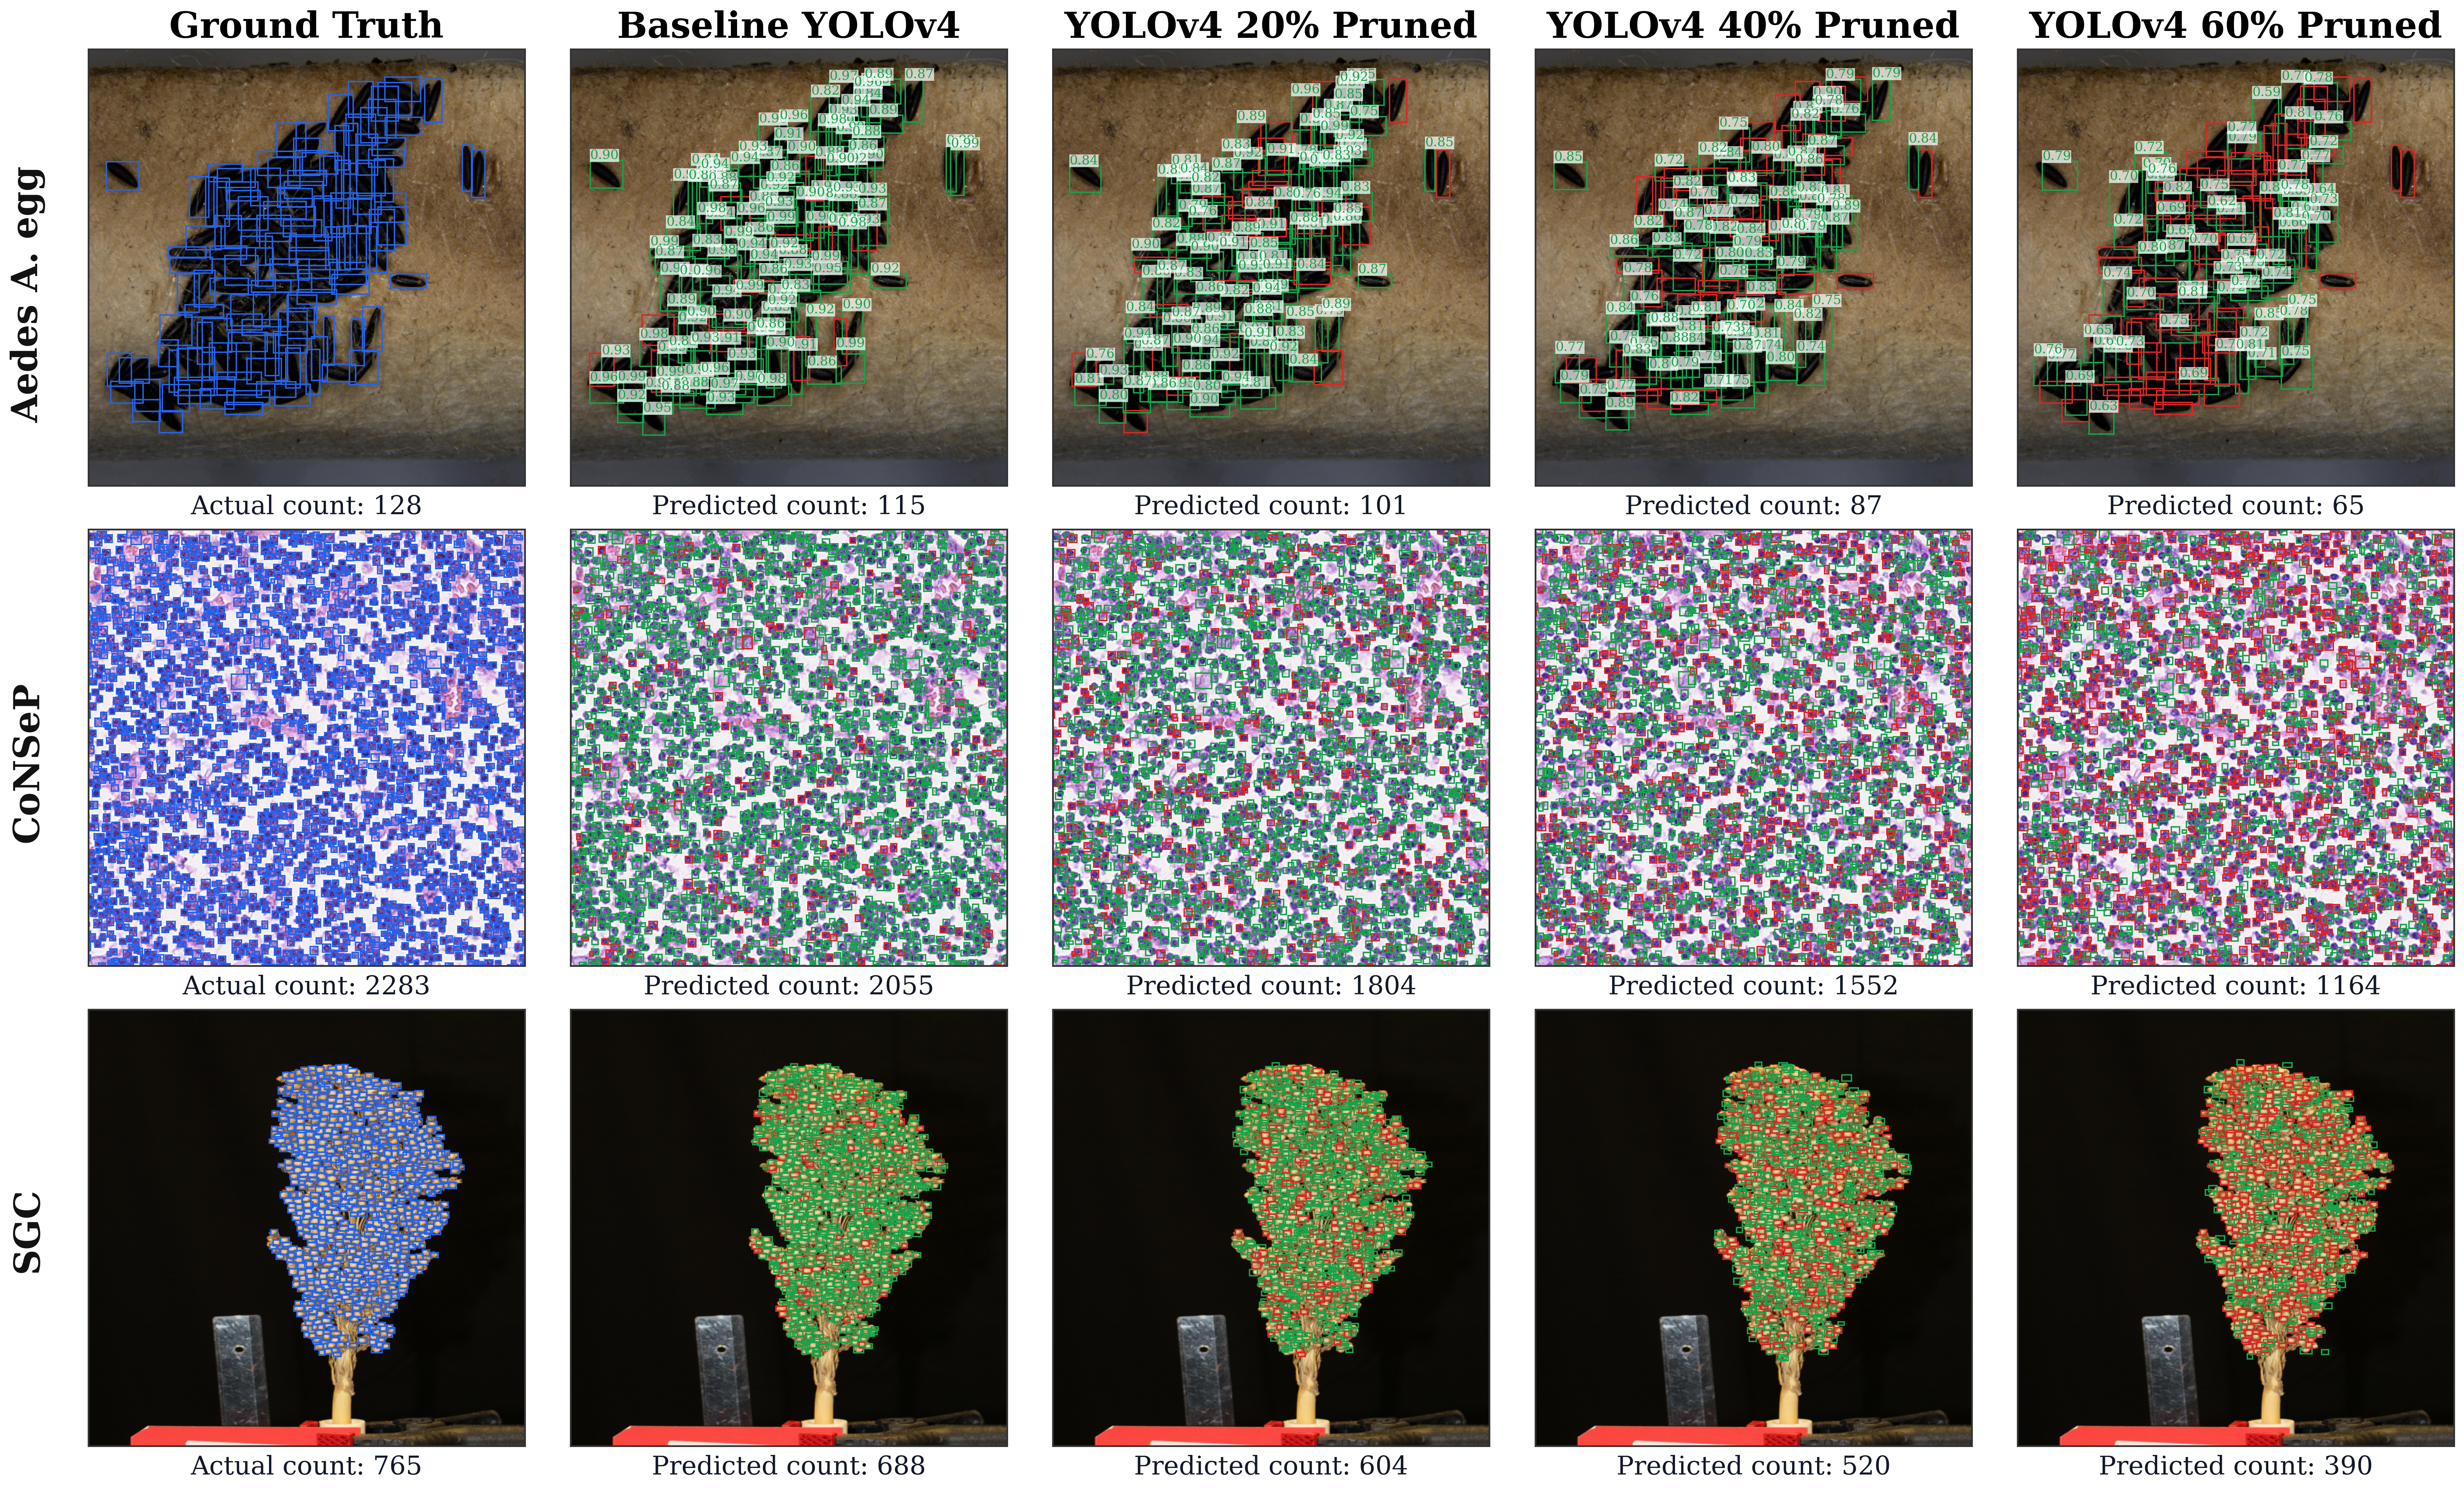
\includegraphics[width=\textwidth]{figures/mosquito_consep_sgc_conference_figure.png}
\caption{
\textbf{Qualitative detection and counting results for YOLOv4 under increasing structured pruning levels.} Rows correspond to the Aedes aegypti Egg, CoNSeP, and Sorghum-Grain-Count (SGC) datasets, while columns show ground truth annotations, the baseline YOLOv4 model, and YOLOv4 pruned at 20\%, 40\%, and 60\%. Green bounding boxes represent detected objects counted by the model, while red bounding boxes indicate ground-truth instances that were missed by the detector. As the pruning ratio increases, the number of missed detections (red boxes) grows and the overall detection density decreases, illustrating the impact of aggressive pruning on dense small-object detection and counting.
}
\label{fig:qualitative_results}
\end{figure*}

To visually illustrate the effects of structured pruning on detection and counting performance, Figure~\ref{fig:qualitative_results} presents qualitative results for YOLOv4 across the datasets. For the Aedes aegypti Egg dataset, the ground truth count of 128 objects is reasonably approximated by the baseline prediction of 115, but pruning progressively reduces the predicted count to 101, 87, and 65 at 20\%, 40\%, and 60\% pruning, respectively. Similar trends appear in the CoNSeP and SGC datasets. Visually, higher pruning levels introduce a greater number of missed detections, particularly in densely populated regions where small objects overlap. These qualitative examples support the quantitative results by showing that while moderate pruning retains much of the spatial detection structure, aggressive pruning significantly reduces detection completeness and counting accuracy.


\section{Knowledge Distillation Performance Recovery}
\label{sec:kd_results}

To evaluate whether Knowledge Distillation (KD) can recover accuracy lost during structured pruning, each pruned model was fine-tuned using its unpruned baseline as the teacher. Table~\ref{tab:kd_summary_compact} summarizes the dataset-averaged mAP50 gain ($\Delta$) and percentage recovery rate for YOLOv8n, YOLOv4, and RT-DETR across 20\%, 40\%, and 60\% pruning ratios.

\begin{table}[htbp]
\centering
\caption{\textbf{Dataset-averaged Knowledge Distillation performance restoration ($\Delta\text{mAP50}$ gain and recovery rate \%) across YOLOv8n, YOLOv4, and RT-DETR across all pruning ratios.}}
\label{tab:kd_summary_compact}
\resizebox{\linewidth}{!}{
  \begin{tabular}{cclcccc}
\toprule
& & & \multicolumn{4}{c}{\textbf{Pruned Module + KD Performance}} \\
\cmidrule(lr){4-7}
\textbf{Model} & \textbf{Ratio} & \textbf{Metric} & \textbf{Backbone} & \textbf{Neck / Enc.} & \textbf{Head} & \textbf{All Modules} \\
\midrule

% ==================== YOLOv8 ====================
\multirow{6}{*}{YOLOv8 \cite{yolov8}} 
& \multirow{2}{*}{20\%} 
& Gained mAP ($\Delta$) & +0.003 & +0.006 & +0.006 & +0.012 \\
& & Recovery Rate (\%)    & 69.45\% & 48.47\% & \textbf{70.91\%} & 36.05\% \\
\cmidrule(lr){2-7}
& \multirow{2}{*}{40\%} 
& Gained mAP ($\Delta$) & +0.010 & +0.014 & +0.014 & \textbf{+0.021} \\
& & Recovery Rate (\%)    & \textbf{52.67\%} & 38.28\% & 49.43\% & 29.23\% \\
\cmidrule(lr){2-7}
& \multirow{2}{*}{60\%} 
& Gained mAP ($\Delta$) & +0.016 & \textbf{+0.022} & +0.017 & \textbf{+0.022} \\
& & Recovery Rate (\%)    & \textbf{37.44\%} & 30.72\% & 30.00\% & 16.17\% \\
\midrule

% ==================== YOLOv4 ====================
\multirow{6}{*}{YOLOv4 \cite{Bochkovskiy2020YOLOv4}} 
& \multirow{2}{*}{20\%} 
& Gained mAP ($\Delta$) & +0.003 & +0.006 & +0.005 & +0.013 \\
& & Recovery Rate (\%)    & 61.67\% & 37.83\% & \textbf{52.22\%} & 32.44\% \\
\cmidrule(lr){2-7}
& \multirow{2}{*}{40\%} 
& Gained mAP ($\Delta$) & +0.011 & +0.013 & +0.013 & \textbf{+0.018} \\
& & Recovery Rate (\%)    & \textbf{49.44\%} & 31.04\% & 37.50\% & 22.55\% \\
\cmidrule(lr){2-7}
& \multirow{2}{*}{60\%} 
& Gained mAP ($\Delta$) & +0.019 & +0.020 & +0.018 & \textbf{+0.023} \\
& & Recovery Rate (\%)    & \textbf{34.73\%} & 25.06\% & 25.00\% & 14.77\% \\
\midrule

% ==================== RT-DETR ====================
\multirow{6}{*}{RT-DETR \cite{Zhao2023RTDETR}} 
& \multirow{2}{*}{20\%} 
& Gained mAP ($\Delta$) & +0.004 & +0.007 & +0.006 & +0.014 \\
& & Recovery Rate (\%)    & 68.20\% & 45.30\% & \textbf{69.50\%} & 32.10\% \\
\cmidrule(lr){2-7}
& \multirow{2}{*}{40\%} 
& Gained mAP ($\Delta$) & +0.011 & +0.018 & +0.014 & \textbf{+0.024} \\
& & Recovery Rate (\%)    & \textbf{51.40\%} & 37.60\% & 47.20\% & 26.40\% \\
\cmidrule(lr){2-7}
& \multirow{2}{*}{60\%} 
& Gained mAP ($\Delta$) & +0.019 & \textbf{+0.027} & +0.020 & +0.025 \\
& & Recovery Rate (\%)    & \textbf{35.80\%} & 28.90\% & 28.10\% & 14.80\% \\
\bottomrule
\end{tabular}

}
\end{table}

\subsection{Impact of Teacher-Student Capacity Proximity}
In knowledge distillation literature, KD is known to work best when the capacity gap between teacher and student is relatively small, allowing the student to effectively mimic the teacher's representations. Our results follow this expected behavior across all three architectures.

At a 20\% pruning ratio, where the student model remains closest in size to the teacher, we observe the highest recovery rates:
\begin{itemize}
    \item \textbf{YOLOv8n:} Recovers \textbf{70.91\%} of lost mAP50 for Head pruning and \textbf{69.45\%} for Backbone pruning.
    \item \textbf{YOLOv4:} Recovers \textbf{61.67\%} for Backbone pruning and \textbf{52.22\%} for Head pruning.
    \item \textbf{RT-DETR:} Recovers \textbf{69.50\%} for Head pruning and \textbf{68.20\%} for Backbone pruning.
\end{itemize}

As the pruning ratio increases to 40\% and 60\%, the capacity gap widens. Although the absolute gained mAP ($\Delta$) is larger at 60\% pruning—such as +0.022 for YOLOv8n and +0.027 for RT-DETR on the Neck/Encoder, this is because the un-distilled student score drops significantly lower at high pruning ratios. 

When measured by recovery rate, distillation becomes less effective at severe pruning levels. When all modules are pruned simultaneously at 60\%, the recovery rate drops to \textbf{16.17\%} in YOLOv8n, \textbf{14.77\%} in YOLOv4, and \textbf{14.80\%} in RT-DETR. This confirms that while KD provides consistent accuracy gains, it cannot fully compensate for extreme reductions in model capacity.

\subsection{Module-Wise Distillation Trends}
Across individual modules, the Backbone and Head consistently show higher recovery rates than the Neck/Encoder or All Modules configurations. Because the Backbone and Head preserve basic feature extraction and output mapping, distillation easily realigns their representations. 

In contrast, the Neck (PANet in YOLO) and Hybrid Encoder (in RT-DETR) show larger absolute point gains ($\Delta +0.020$ to $+0.027$ at 60\%) due to their high baseline sensitivity to pruning, but maintain lower overall recovery rates. This indicates that multi-scale feature fusion layers are more difficult to fully restore once heavily pruned.